\chapter{Architecture}

\section{Overview}

\begin{figure}[h]
    \caption{Overview}
    \centering
    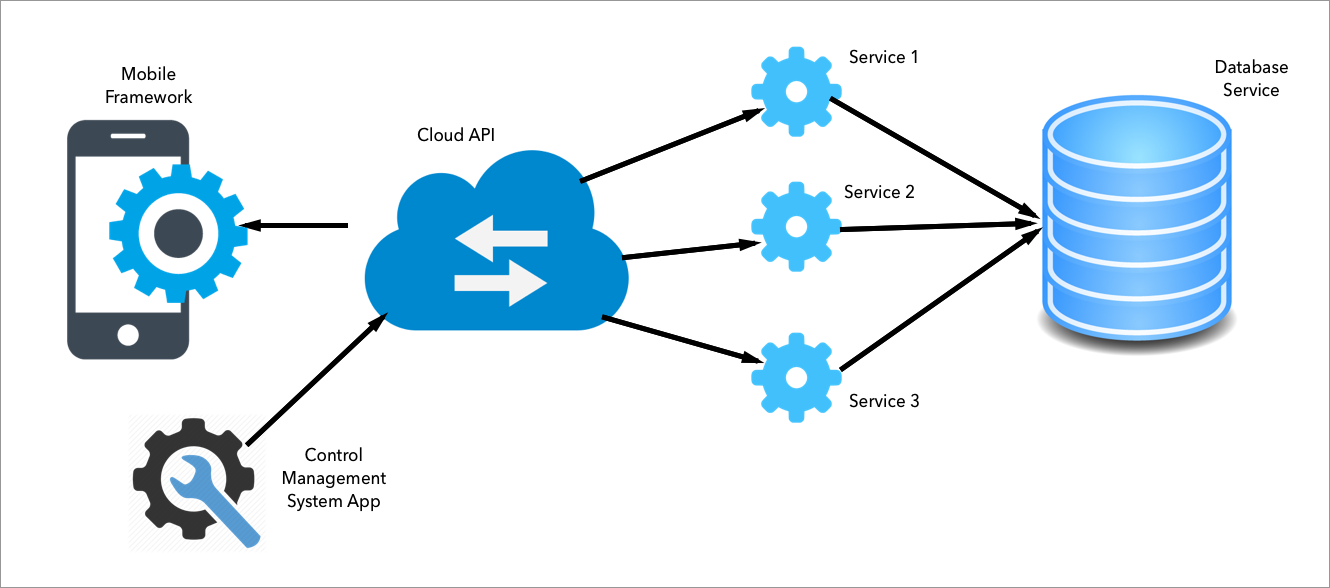
\includegraphics[width=100mm]{images/overview}
    \label{fig:label}
\end{figure}

% Fig 4.1 shows the complete Mobile Back-end as a Service system. It shows the mobile framework used by developers application to send HTTPS request using a REST API such as get request to retrieve objects from the database layer using a service layer. The service layer is where the database, notifications
% and remote configuration services sit. So when a request is made to the Cloud Rest API framework such as send object to the server , the API will call the database service class and will enter the object into the database and return the result back to the client ( framework). The diagram also shows the Control Management System (CMS) app using a dashboard to accomplish such tasks as send the configuration files updates to the server, which will send HTTPS request to the Cloud API and have its own service class to accomplish these tasks. The diagram only displays 3 service class, but can be as many as required.

% Mobile frameworks separates the back-end API by functionality, making it easier for developers to create apps without having to learn how the API works. It provides class functions and protocols to which can be used to interact with the server API. An example of this is in Fig 5.3 where the framework has the database object that makes HTTPS request to retrieve the objects, but the developer can use the inherited function call getObjects. The
% remote configuration requests are also in the diagram to get values from the JSON files stored on the mobile phone app directory.

\section{Back-end as a Service}

\begin{figure}[!h]
    \caption{Client Server Diagram}
    \centering
    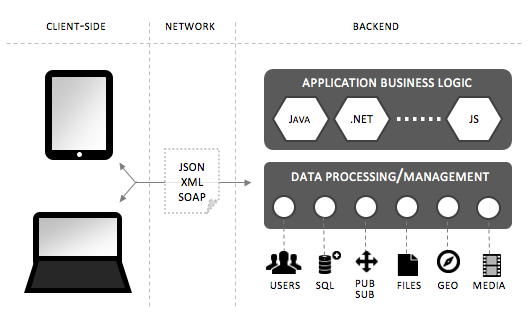
\includegraphics[width=100mm]{images/client-server-diagram}
    \label{fig:client-server}
\end{figure}

Applications today are put into the category of "client-server apps" where the applications consist of client-side(frontend) and the server-side(backend). The client-side is what the user see, what type of device it is, being computer or mobile apps. The client-side is responsibility for show the data to user in some sort of interface, along with taking their requests and passing it to the server. 
The backend consists of two primary components: application business logic and data processing/management. The data processing/management operates on various resources being users, persistent data, files etc. The business logic manages triggering notifications based on changes in the data, prevent unauthorised access.  Figure \ref{fig:client-server} illustrates this.

\subsection{API}

In order for the applications to communicate with the back-end, there needs to be a common based protocol that defines how data flows. Thus combining the protocol with the data structure definitions created an Application Programming Interface (API). The typical format used in most applications is called  Representational State Transfer REST which is an architectural style and approach to communications used in web services development. REST provides a list of verbs such as GET, POST, DELETE in which request can be made using HTTP. The diagram \ref{fig:api} below illustrates this: 

\begin{figure}[!h]
    \caption{API}
    \centering
    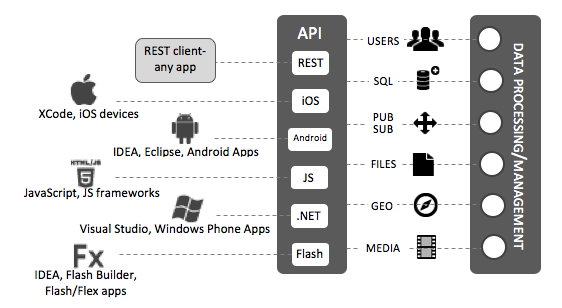
\includegraphics[width=100mm]{images/baas-apis}
    \label{fig:api}
\end{figure}


\section{Methodologies}


\section{Main part of MBaaS}

As stated from Kinvey \cite{kinveywebsite} there are five key parts what the architecture should cover. These include the following:

\begin{itemize}
  \item Mobile is driving the adoption of cloud in the enterprise
    - to include cloud-based data delivery, with flexibility to run on public and private clouds
  \item Enable agility with security
    - the needs to blend developers launching apps quickly along with still be secure
  \item Ensure secure, compliant app use
    - the architecture needs to monitor data on in the network, allowing access to only authorized requests
  \item Hardware/ Platform flexibility 
    - the apps needs to run on all platforms
\end{itemize}
